\PassOptionsToPackage{unicode=true}{hyperref} % options for packages loaded elsewhere
\PassOptionsToPackage{hyphens}{url}
%
\documentclass[ignorenonframetext,]{beamer}
\usebackgroundtemplate{%
\includegraphics[width=\paperwidth]{url(\url{https://github.com/yihui/xaringan/releases/download/v0.0.2/karl-moustache.jpg})}%
}
\usepackage{pgfpages}
\setbeamertemplate{caption}[numbered]
\setbeamertemplate{caption label separator}{: }
\setbeamercolor{caption name}{fg=normal text.fg}
\beamertemplatenavigationsymbolsempty
\usepackage{lmodern}
\usepackage{amssymb,amsmath}
\usepackage{ifxetex,ifluatex}
\usepackage{fixltx2e} % provides \textsubscript
\ifnum 0\ifxetex 1\fi\ifluatex 1\fi=0 % if pdftex
  \usepackage[T1]{fontenc}
  \usepackage[utf8]{inputenc}
  \usepackage{textcomp} % provides euro and other symbols
\else % if luatex or xelatex
  \usepackage{unicode-math}
  \defaultfontfeatures{Ligatures=TeX,Scale=MatchLowercase}
\fi
\usetheme[]{AnnArbor}
\usecolortheme{dolphin}
\usefonttheme{structurebold}
% use upquote if available, for straight quotes in verbatim environments
\IfFileExists{upquote.sty}{\usepackage{upquote}}{}
% use microtype if available
\IfFileExists{microtype.sty}{%
\usepackage[]{microtype}
\UseMicrotypeSet[protrusion]{basicmath} % disable protrusion for tt fonts
}{}
\IfFileExists{parskip.sty}{%
\usepackage{parskip}
}{% else
\setlength{\parindent}{0pt}
\setlength{\parskip}{6pt plus 2pt minus 1pt}
}
\usepackage{hyperref}
\hypersetup{
            pdftitle={Presentation Ninja},
            pdfauthor={Yihui Xie},
            pdfborder={0 0 0},
            breaklinks=true}
\urlstyle{same}  % don't use monospace font for urls
\newif\ifbibliography
\usepackage{color}
\usepackage{fancyvrb}
\newcommand{\VerbBar}{|}
\newcommand{\VERB}{\Verb[commandchars=\\\{\}]}
\DefineVerbatimEnvironment{Highlighting}{Verbatim}{commandchars=\\\{\}}
% Add ',fontsize=\small' for more characters per line
\usepackage{framed}
\definecolor{shadecolor}{RGB}{248,248,248}
\newenvironment{Shaded}{\begin{snugshade}}{\end{snugshade}}
\newcommand{\AlertTok}[1]{\textcolor[rgb]{0.94,0.16,0.16}{#1}}
\newcommand{\AnnotationTok}[1]{\textcolor[rgb]{0.56,0.35,0.01}{\textbf{\textit{#1}}}}
\newcommand{\AttributeTok}[1]{\textcolor[rgb]{0.77,0.63,0.00}{#1}}
\newcommand{\BaseNTok}[1]{\textcolor[rgb]{0.00,0.00,0.81}{#1}}
\newcommand{\BuiltInTok}[1]{#1}
\newcommand{\CharTok}[1]{\textcolor[rgb]{0.31,0.60,0.02}{#1}}
\newcommand{\CommentTok}[1]{\textcolor[rgb]{0.56,0.35,0.01}{\textit{#1}}}
\newcommand{\CommentVarTok}[1]{\textcolor[rgb]{0.56,0.35,0.01}{\textbf{\textit{#1}}}}
\newcommand{\ConstantTok}[1]{\textcolor[rgb]{0.00,0.00,0.00}{#1}}
\newcommand{\ControlFlowTok}[1]{\textcolor[rgb]{0.13,0.29,0.53}{\textbf{#1}}}
\newcommand{\DataTypeTok}[1]{\textcolor[rgb]{0.13,0.29,0.53}{#1}}
\newcommand{\DecValTok}[1]{\textcolor[rgb]{0.00,0.00,0.81}{#1}}
\newcommand{\DocumentationTok}[1]{\textcolor[rgb]{0.56,0.35,0.01}{\textbf{\textit{#1}}}}
\newcommand{\ErrorTok}[1]{\textcolor[rgb]{0.64,0.00,0.00}{\textbf{#1}}}
\newcommand{\ExtensionTok}[1]{#1}
\newcommand{\FloatTok}[1]{\textcolor[rgb]{0.00,0.00,0.81}{#1}}
\newcommand{\FunctionTok}[1]{\textcolor[rgb]{0.00,0.00,0.00}{#1}}
\newcommand{\ImportTok}[1]{#1}
\newcommand{\InformationTok}[1]{\textcolor[rgb]{0.56,0.35,0.01}{\textbf{\textit{#1}}}}
\newcommand{\KeywordTok}[1]{\textcolor[rgb]{0.13,0.29,0.53}{\textbf{#1}}}
\newcommand{\NormalTok}[1]{#1}
\newcommand{\OperatorTok}[1]{\textcolor[rgb]{0.81,0.36,0.00}{\textbf{#1}}}
\newcommand{\OtherTok}[1]{\textcolor[rgb]{0.56,0.35,0.01}{#1}}
\newcommand{\PreprocessorTok}[1]{\textcolor[rgb]{0.56,0.35,0.01}{\textit{#1}}}
\newcommand{\RegionMarkerTok}[1]{#1}
\newcommand{\SpecialCharTok}[1]{\textcolor[rgb]{0.00,0.00,0.00}{#1}}
\newcommand{\SpecialStringTok}[1]{\textcolor[rgb]{0.31,0.60,0.02}{#1}}
\newcommand{\StringTok}[1]{\textcolor[rgb]{0.31,0.60,0.02}{#1}}
\newcommand{\VariableTok}[1]{\textcolor[rgb]{0.00,0.00,0.00}{#1}}
\newcommand{\VerbatimStringTok}[1]{\textcolor[rgb]{0.31,0.60,0.02}{#1}}
\newcommand{\WarningTok}[1]{\textcolor[rgb]{0.56,0.35,0.01}{\textbf{\textit{#1}}}}
\usepackage{graphicx,grffile}
\makeatletter
\def\maxwidth{\ifdim\Gin@nat@width>\linewidth\linewidth\else\Gin@nat@width\fi}
\def\maxheight{\ifdim\Gin@nat@height>\textheight\textheight\else\Gin@nat@height\fi}
\makeatother
% Scale images if necessary, so that they will not overflow the page
% margins by default, and it is still possible to overwrite the defaults
% using explicit options in \includegraphics[width, height, ...]{}
\setkeys{Gin}{width=\maxwidth,height=\maxheight,keepaspectratio}
% Prevent slide breaks in the middle of a paragraph:
\widowpenalties 1 10000
\raggedbottom
\setbeamertemplate{part page}{
\centering
\begin{beamercolorbox}[sep=16pt,center]{part title}
  \usebeamerfont{part title}\insertpart\par
\end{beamercolorbox}
}
\setbeamertemplate{section page}{
\centering
\begin{beamercolorbox}[sep=12pt,center]{part title}
  \usebeamerfont{section title}\insertsection\par
\end{beamercolorbox}
}
\setbeamertemplate{subsection page}{
\centering
\begin{beamercolorbox}[sep=8pt,center]{part title}
  \usebeamerfont{subsection title}\insertsubsection\par
\end{beamercolorbox}
}
\AtBeginPart{
  \frame{\partpage}
}
\AtBeginSection{
  \ifbibliography
  \else
    \frame{\sectionpage}
  \fi
}
\AtBeginSubsection{
  \frame{\subsectionpage}
}
\setlength{\emergencystretch}{3em}  % prevent overfull lines
\providecommand{\tightlist}{%
  \setlength{\itemsep}{0pt}\setlength{\parskip}{0pt}}
\setcounter{secnumdepth}{0}

% set default figure placement to htbp
\makeatletter
\def\fps@figure{htbp}
\makeatother


\title{Presentation Ninja}
\providecommand{\subtitle}[1]{}
\subtitle{⚔with xaringan}
\author{Yihui Xie}
\date{2016/12/12 (updated: 2018-09-26)}

\begin{document}
\frame{\titlepage}

\begin{frame}

background-image:
url(\url{https://upload.wikimedia.org/wikipedia/commons/b/be/Sharingan_triple.svg})

???

Image credit:
\href{https://commons.wikimedia.org/wiki/File:Sharingan_triple.svg}{Wikimedia
Commons}

class: inverse, center, middle

\end{frame}

\begin{frame}{Get Started}
\protect\hypertarget{get-started}{}

\end{frame}

\begin{frame}[fragile]{Hello World}
\protect\hypertarget{hello-world}{}

Install the \textbf{xaringan} package from
\href{https://github.com/yihui/xaringan}{Github}:

\begin{Shaded}
\begin{Highlighting}[]
\NormalTok{devtools}\OperatorTok{::}\KeywordTok{install_github}\NormalTok{(}\StringTok{"yihui/xaringan"}\NormalTok{)}
\end{Highlighting}
\end{Shaded}

--

You are recommended to use the
\href{https://www.rstudio.com/products/rstudio/}{RStudio IDE}, but you
do not have to.

\begin{itemize}
\tightlist
\item
  Create a new R Markdown document from the menu
  \texttt{File\ -\textgreater{}\ New\ File\ -\textgreater{}\ R\ Markdown\ -\textgreater{}\ From\ Template\ -\textgreater{}\ Ninja\ Presentation};1
\end{itemize}

--

\begin{itemize}
\tightlist
\item
  Click the \texttt{Knit} button to compile it;
\end{itemize}

--

\begin{itemize}
\tightlist
\item
  or use the \href{https://rstudio.github.io/rstudioaddins/}{RStudio
  Addin}2 ``Infinite Moon Reader'' to live preview the slides (every
  time you update and save the Rmd document, the slides will be
  automatically reloaded in RStudio Viewer.
\end{itemize}

.footnote{[} {[}1{]}
中文用户请看\href{http://slides.yihui.name/xaringan/zh-CN.html}{这份教程}

{[}2{]} See \href{https://github.com/yihui/xaringan/issues/2}{\#2} if
you do not see the template or addin in RStudio. {]}

\end{frame}

\begin{frame}{Hello Ninja}
\protect\hypertarget{hello-ninja}{}

As a presentation ninja, you certainly should not be satisfied by the
``Hello World'' example. You need to understand more about two things:

\begin{enumerate}
\item
  The \href{https://remarkjs.com}{remark.js} library;
\item
  The \textbf{xaringan} package;
\end{enumerate}

Basically \textbf{xaringan} injected the chakra of R Markdown (minus
Pandoc) into \textbf{remark.js}. The slides are rendered by remark.js in
the web browser, and the Markdown source needed by remark.js is
generated from R Markdown (\textbf{knitr}).

\end{frame}

\begin{frame}{remark.js}
\protect\hypertarget{remark.js}{}

You can see an introduction of remark.js from
\href{https://remarkjs.com}{its homepage}. You should read the
\href{https://github.com/gnab/remark/wiki}{remark.js Wiki} at least once
to know how to

\begin{itemize}
\item
  create a new slide (Markdown syntax* and slide properties);
\item
  format a slide (e.g.~text alignment);
\item
  configure the slideshow;
\item
  and use the presentation (keyboard shortcuts).
\end{itemize}

It is important to be familiar with remark.js before you can understand
the options in \textbf{xaringan}.

.footnote{[}{[}*{]} It is different with Pandoc's Markdown! It is
limited but should be enough for presentation purposes. Come on\ldots{}
You do not need a slide for the Table of Contents! Well, the Markdown
support in remark.js
\href{https://github.com/gnab/remark/issues/142}{may be improved} in the
future.{]}

class: inverse, middle, center

\end{frame}

\begin{frame}{Using xaringan}
\protect\hypertarget{using-xaringan}{}

\end{frame}

\begin{frame}[fragile]{xaringan}
\protect\hypertarget{xaringan}{}

Provides an R Markdown output format \texttt{xaringan::moon\_reader} as
a wrapper for remark.js, and you can use it in the YAML metadata, e.g.

\begin{Shaded}
\begin{Highlighting}[]
\OtherTok{---}
\FunctionTok{title:}\AttributeTok{ }\StringTok{"A Cool Presentation"}
\FunctionTok{output:}
  \FunctionTok{xaringan:}\AttributeTok{:moon_reader}
    \FunctionTok{yolo:}\AttributeTok{ true}
    \FunctionTok{nature:}
      \FunctionTok{autoplay:}\AttributeTok{ 30000}
\OtherTok{---}
\end{Highlighting}
\end{Shaded}

See the help page \texttt{?xaringan::moon\_reader} for all possible
options that you can use.

\end{frame}

\begin{frame}[fragile]{remark.js vs xaringan}
\protect\hypertarget{remark.js-vs-xaringan}{}

Some differences between using remark.js (left) and using
\textbf{xaringan} (right):

.pull-left{[} 1. Start with a boilerplate HTML file;

\begin{enumerate}
\item
  Plain Markdown;
\item
  Write JavaScript to autoplay slides;
\item
  Manually configure MathJax;
\item
  Highlight code with \texttt{*};
\item
  Edit Markdown source and refresh browser to see updated slides; {]}
\end{enumerate}

.pull-right{[} 1. Start with an R Markdown document;

\begin{enumerate}
\item
  R Markdown (can embed R/other code chunks);
\item
  Provide an option \texttt{autoplay};
\item
  MathJax just works;*
\item
  Highlight code with \texttt{\{\{\}\}};
\item
  The RStudio addin ``Infinite Moon Reader'' automatically refreshes
  slides on changes; {]}
\end{enumerate}

.footnote{[}{[}*{]} Not really. See next page.{]}

\end{frame}

\begin{frame}[fragile]{Math Expressions}
\protect\hypertarget{math-expressions}{}

You can write LaTeX math expressions inside a pair of dollar signs, e.g.
\$\alpha+\beta\$ renders \(\alpha+\beta\). You can use the display style
with double dollar signs:

\begin{verbatim}
$$\bar{X}=\frac{1}{n}\sum_{i=1}^nX_i$$
\end{verbatim}

\[\bar{X}=\frac{1}{n}\sum_{i=1}^nX_i\]

Limitations:

\begin{enumerate}
\item
  The source code of a LaTeX math expression must be in one line, unless
  it is inside a pair of double dollar signs, in which case the starting
  \texttt{\$\$} must appear in the very beginning of a line, followed
  immediately by a non-space character, and the ending \texttt{\$\$}
  must be at the end of a line, led by a non-space character;
\item
  There should not be spaces after the opening \texttt{\$} or before the
  closing \texttt{\$}.
\item
  Math does not work on the title slide (see
  \href{https://github.com/yihui/xaringan/issues/61}{\#61} for a
  workaround).
\end{enumerate}

\end{frame}

\begin{frame}[fragile]{R Code}
\protect\hypertarget{r-code}{}

\begin{Shaded}
\begin{Highlighting}[]
\CommentTok{# a boring regression}
\NormalTok{fit =}\StringTok{ }\KeywordTok{lm}\NormalTok{(dist }\OperatorTok{~}\StringTok{ }\DecValTok{1} \OperatorTok{+}\StringTok{ }\NormalTok{speed, }\DataTypeTok{data =}\NormalTok{ cars)}
\KeywordTok{coef}\NormalTok{(}\KeywordTok{summary}\NormalTok{(fit))}
\end{Highlighting}
\end{Shaded}

\begin{verbatim}
#               Estimate Std. Error   t value     Pr(>|t|)
# (Intercept) -17.579095  6.7584402 -2.601058 1.231882e-02
# speed         3.932409  0.4155128  9.463990 1.489836e-12
\end{verbatim}

\begin{Shaded}
\begin{Highlighting}[]
\NormalTok{dojutsu =}\StringTok{ }\KeywordTok{c}\NormalTok{(}\StringTok{'地爆天星'}\NormalTok{, }\StringTok{'天照'}\NormalTok{, }\StringTok{'加具土命'}\NormalTok{, }\StringTok{'神威'}\NormalTok{, }\StringTok{'須佐能乎'}\NormalTok{, }\StringTok{'無限月読'}\NormalTok{)}
\KeywordTok{grep}\NormalTok{(}\StringTok{'天'}\NormalTok{, dojutsu, }\DataTypeTok{value =} \OtherTok{TRUE}\NormalTok{)}
\end{Highlighting}
\end{Shaded}

\begin{verbatim}
# [1] "地爆天星" "天照"
\end{verbatim}

\end{frame}

\begin{frame}[fragile]{R Plots}
\protect\hypertarget{r-plots}{}

\begin{Shaded}
\begin{Highlighting}[]
\KeywordTok{par}\NormalTok{(}\DataTypeTok{mar =} \KeywordTok{c}\NormalTok{(}\DecValTok{4}\NormalTok{, }\DecValTok{4}\NormalTok{, }\DecValTok{1}\NormalTok{, }\FloatTok{.1}\NormalTok{))}
\KeywordTok{plot}\NormalTok{(cars, }\DataTypeTok{pch =} \DecValTok{19}\NormalTok{, }\DataTypeTok{col =} \StringTok{'darkgray'}\NormalTok{, }\DataTypeTok{las =} \DecValTok{1}\NormalTok{)}
\KeywordTok{abline}\NormalTok{(fit, }\DataTypeTok{lwd =} \DecValTok{2}\NormalTok{)}
\end{Highlighting}
\end{Shaded}

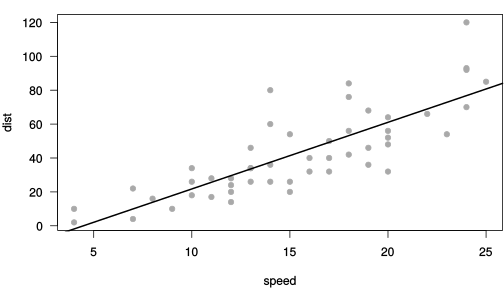
\includegraphics{slides_files/figure-beamer/cars-1.svg}

\end{frame}

\begin{frame}[fragile]{Tables}
\protect\hypertarget{tables}{}

If you want to generate a table, make sure it is in the HTML format
(instead of Markdown or other formats), e.g.,

\begin{Shaded}
\begin{Highlighting}[]
\NormalTok{knitr}\OperatorTok{::}\KeywordTok{kable}\NormalTok{(}\KeywordTok{head}\NormalTok{(iris), }\DataTypeTok{format =} \StringTok{'html'}\NormalTok{)}
\end{Highlighting}
\end{Shaded}

Sepal.Length

Sepal.Width

Petal.Length

Petal.Width

Species

5.1

3.5

1.4

0.2

setosa

4.9

3.0

1.4

0.2

setosa

4.7

3.2

1.3

0.2

setosa

4.6

3.1

1.5

0.2

setosa

5.0

3.6

1.4

0.2

setosa

5.4

3.9

1.7

0.4

setosa

\end{frame}

\begin{frame}[fragile]{HTML Widgets}
\protect\hypertarget{html-widgets}{}

I have not thoroughly tested HTML widgets against \textbf{xaringan}.
Some may work well, and some may not. It is a little tricky.

Similarly, the Shiny mode (\texttt{runtime:\ shiny}) does not work. I
might get these issues fixed in the future, but these are not of high
priority to me. I never turn my presentation into a Shiny app. When I
need to demonstrate more complicated examples, I just launch them
separately. It is convenient to share slides with other people when they
are plain HTML/JS applications.

See the next page for two HTML widgets.

\end{frame}

\begin{frame}[fragile]

\begin{Shaded}
\begin{Highlighting}[]
\KeywordTok{library}\NormalTok{(leaflet)}
\KeywordTok{leaflet}\NormalTok{() }\OperatorTok\StringTok{ }\KeywordTok{addTiles}\NormalTok{() }\OperatorTok\StringTok{ }\KeywordTok{setView}\NormalTok{(}\OperatorTok{-}\FloatTok{93.65}\NormalTok{, }\FloatTok{42.0285}\NormalTok{, }\DataTypeTok{zoom =} \DecValTok{17}\NormalTok{)}
\end{Highlighting}
\end{Shaded}

\end{frame}

\begin{frame}[fragile]

\begin{Shaded}
\begin{Highlighting}[]
\NormalTok{DT}\OperatorTok{::}\KeywordTok{datatable}\NormalTok{(}
  \KeywordTok{head}\NormalTok{(iris, }\DecValTok{10}\NormalTok{),}
  \DataTypeTok{fillContainer =} \OtherTok{FALSE}\NormalTok{, }\DataTypeTok{options =} \KeywordTok{list}\NormalTok{(}\DataTypeTok{pageLength =} \DecValTok{8}\NormalTok{)}
\NormalTok{)}
\end{Highlighting}
\end{Shaded}

\end{frame}

\begin{frame}[fragile]{Some Tips}
\protect\hypertarget{some-tips}{}

\begin{itemize}
\item
  When you use the ``Infinite Moon Reader'' addin in RStudio, your R
  session will be blocked by default. You can click the red button on
  the right of the console to stop serving the slides, or use the
  \emph{daemonized} mode so that it does not block your R session. To do
  the latter, you can set the option

\begin{Shaded}
\begin{Highlighting}[]
\KeywordTok{options}\NormalTok{(}\DataTypeTok{servr.daemon =} \OtherTok{TRUE}\NormalTok{)}
\end{Highlighting}
\end{Shaded}

  in your current R session, or in \texttt{\textasciitilde{}/.Rprofile}
  so that it is applied to all future R sessions. I do the latter by
  myself.

  To know more about the web server, see the
  \href{https://github.com/yihui/servr}{\textbf{servr}} package.
\end{itemize}

--

\begin{itemize}
\item
  Do not forget to try the \texttt{yolo} option of
  \texttt{xaringan::moon\_reader}.

\begin{Shaded}
\begin{Highlighting}[]
\FunctionTok{output:}
  \FunctionTok{xaringan:}\AttributeTok{:moon_reader:}
    \FunctionTok{yolo:}\AttributeTok{ true}
\end{Highlighting}
\end{Shaded}
\end{itemize}

\end{frame}

\begin{frame}[fragile]{Some Tips}
\protect\hypertarget{some-tips-1}{}

\begin{itemize}
\item
  Slides can be automatically played if you set the \texttt{autoplay}
  option under \texttt{nature}, e.g.~go to the next slide every 30
  seconds in a lightning talk:

\begin{Shaded}
\begin{Highlighting}[]
\FunctionTok{output:}
  \FunctionTok{xaringan:}\AttributeTok{:moon_reader:}
    \FunctionTok{nature:}
      \FunctionTok{autoplay:}\AttributeTok{ 30000}
\end{Highlighting}
\end{Shaded}
\end{itemize}

--

\begin{itemize}
\item
  A countdown timer can be added to every page of the slides using the
  \texttt{countdown} option under \texttt{nature}, e.g.~if you want to
  spend one minute on every page when you give the talk, you can set:

\begin{Shaded}
\begin{Highlighting}[]
\FunctionTok{output:}
  \FunctionTok{xaringan:}\AttributeTok{:moon_reader:}
    \FunctionTok{nature:}
      \FunctionTok{countdown:}\AttributeTok{ 60000}
\end{Highlighting}
\end{Shaded}

  Then you will see a timer counting down from \texttt{01:00}, to
  \texttt{00:59}, \texttt{00:58}, \ldots{} When the time is out, the
  timer will continue but the time turns red.
\end{itemize}

\end{frame}

\begin{frame}[fragile]{Some Tips}
\protect\hypertarget{some-tips-2}{}

\begin{itemize}
\item
  The title slide is created automatically by \textbf{xaringan}, but it
  is just another remark.js slide added before your other slides.

  The title slide is set to
  \texttt{class:\ center,\ middle,\ inverse,\ title-slide} by default.
  You can change the classes applied to the title slide with the
  \texttt{titleSlideClass} option of \texttt{nature}
  (\texttt{title-slide} is always applied).

\begin{Shaded}
\begin{Highlighting}[]
\FunctionTok{output:}
  \FunctionTok{xaringan:}\AttributeTok{:moon_reader:}
    \FunctionTok{nature:}
      \FunctionTok{titleSlideClass:}\AttributeTok{ }\KeywordTok{[}\NormalTok{top}\KeywordTok{,}\NormalTok{ left}\KeywordTok{,}\NormalTok{ inverse}\KeywordTok{]}
\end{Highlighting}
\end{Shaded}
\end{itemize}

--

\begin{itemize}
\item
  If you'd like to create your own title slide, disable
  \textbf{xaringan}'s title slide with the \texttt{seal\ =\ FALSE}
  option of \texttt{moon\_reader}.

\begin{Shaded}
\begin{Highlighting}[]
\FunctionTok{output:}
  \FunctionTok{xaringan:}\AttributeTok{:moon_reader:}
    \FunctionTok{seal:}\AttributeTok{ false}
\end{Highlighting}
\end{Shaded}
\end{itemize}

\end{frame}

\begin{frame}[fragile]{Some Tips}
\protect\hypertarget{some-tips-3}{}

\begin{itemize}
\item
  There are several ways to build incremental slides. See
  \href{https://slides.yihui.name/xaringan/incremental.html}{this
  presentation} for examples.
\item
  The option \texttt{highlightLines:\ true} of \texttt{nature} will
  highlight code lines that start with \texttt{*}, or are wrapped in
  \texttt{\{\{\ \}\}}, or have trailing comments
  \texttt{\#\textless{}\textless{}};

\begin{Shaded}
\begin{Highlighting}[]
\FunctionTok{output:}
  \FunctionTok{xaringan:}\AttributeTok{:moon_reader:}
    \FunctionTok{nature:}
      \FunctionTok{highlightLines:}\AttributeTok{ true}
\end{Highlighting}
\end{Shaded}

  See examples on the next page.
\end{itemize}

\end{frame}

\begin{frame}[fragile]{Some Tips}
\protect\hypertarget{some-tips-4}{}

.pull-left{[} An example using a leading \texttt{*}:

\texttt{r\ \ \ \ \ if\ (TRUE)\ \{\ \ \ \ \ **\ message("Very\ important!")\ \ \ \ \ \}}
Output:

\begin{Shaded}
\begin{Highlighting}[]
\ControlFlowTok{if}\NormalTok{ (}\OtherTok{TRUE}\NormalTok{) \{}
\OperatorTok{*}\StringTok{ }\KeywordTok{message}\NormalTok{(}\StringTok{"Very important!"}\NormalTok{)}
\NormalTok{\}}
\end{Highlighting}
\end{Shaded}

This is invalid R code, so it is a plain fenced code block that is not
executed. {]}

.pull-right{[} An example using \texttt{\{\{\}\}}:

\texttt{\{r\ tidy=FALSE\}\ \ \ \ \ if\ (TRUE)\ \{\ \ \ \ \ *\{\{\ message("Very\ important!")\ \}\}\ \ \ \ \ \}}
Output:

\begin{Shaded}
\begin{Highlighting}[]
\ControlFlowTok{if}\NormalTok{ (}\OtherTok{TRUE}\NormalTok{) \{}
\NormalTok{\{\{ }\KeywordTok{message}\NormalTok{(}\StringTok{"Very important!"}\NormalTok{) \}\}}
\NormalTok{\}}
\end{Highlighting}
\end{Shaded}

\begin{verbatim}
## Very important!
\end{verbatim}

It is valid R code so you can run it. Note that \texttt{\{\{\}\}} can
wrap an R expression of multiple lines. {]}

\end{frame}

\begin{frame}[fragile]{Some Tips}
\protect\hypertarget{some-tips-5}{}

An example of using the trailing comment
\texttt{\#\textless{}\textless{}} to highlight lines:

\begin{Shaded}
\begin{Highlighting}[]
\BaseNTok{```\{r tidy=FALSE\}}
\BaseNTok{library(ggplot2)}
\BaseNTok{ggplot(mtcars) + }
\BaseNTok{  aes(mpg, disp) + }
\BaseNTok{  geom_point() +   #<<}
\BaseNTok{  geom_smooth()    #<<}
\BaseNTok{```}
\end{Highlighting}
\end{Shaded}

Output:

\begin{Shaded}
\begin{Highlighting}[]
\KeywordTok{library}\NormalTok{(ggplot2)}
\KeywordTok{ggplot}\NormalTok{(mtcars) }\OperatorTok{+}\StringTok{ }
\StringTok{  }\KeywordTok{aes}\NormalTok{(mpg, disp) }\OperatorTok{+}\StringTok{ }
\StringTok{  }\KeywordTok{geom_point}\NormalTok{() }\OperatorTok{+}\StringTok{   }\CommentTok{#<<}
\StringTok{  }\KeywordTok{geom_smooth}\NormalTok{()    }\CommentTok{#<<}
\end{Highlighting}
\end{Shaded}

\end{frame}

\begin{frame}[fragile]{Some Tips}
\protect\hypertarget{some-tips-6}{}

\begin{itemize}
\item
  To make slides work offline, you need to download a copy of remark.js
  in advance, because \textbf{xaringan} uses the online version by
  default (see the help page \texttt{?xaringan::moon\_reader}).
\item
  You can use \texttt{xaringan::summon\_remark()} to download the latest
  or a specified version of remark.js. By default, it is downloaded to
  \texttt{libs/remark-latest.min.js}.
\item
  Then change the \texttt{chakra} option in YAML to point to this file,
  e.g.

\begin{Shaded}
\begin{Highlighting}[]
\FunctionTok{output:}
  \FunctionTok{xaringan:}\AttributeTok{:moon_reader:}
    \FunctionTok{chakra:}\AttributeTok{ libs/remark-latest.min.js}
\end{Highlighting}
\end{Shaded}
\item
  If you used Google fonts in slides (the default theme uses
  \emph{Yanone Kaffeesatz}, \emph{Droid Serif}, and \emph{Source Code
  Pro}), they won't work offline unless you download or install them
  locally. The Heroku app
  \href{https://google-webfonts-helper.herokuapp.com/fonts}{google-webfonts-helper}
  can help you download fonts and generate the necessary CSS.
\end{itemize}

\end{frame}

\begin{frame}[fragile]{Macros}
\protect\hypertarget{macros}{}

\begin{itemize}
\item
  remark.js \href{https://github.com/yihui/xaringan/issues/80}{allows
  users to define custom macros} (JS functions) that can be applied to
  Markdown text using the syntax
  \texttt{!{[}:macroName\ arg1,\ arg2,\ ...{]}} or
  \texttt{!{[}:macroName\ arg1,\ arg2,\ ...{]}(this)}. For example,
  before remark.js initializes the slides, you can define a macro named
  \texttt{scale}:

\begin{Shaded}
\begin{Highlighting}[]
\VariableTok{remark}\NormalTok{.}\VariableTok{macros}\NormalTok{.}\AttributeTok{scale} \OperatorTok{=} \KeywordTok{function}\NormalTok{ (percentage) }\OperatorTok{\{}
  \KeywordTok{var}\NormalTok{ url }\OperatorTok{=} \KeywordTok{this}\OperatorTok{;}
  \ControlFlowTok{return} \StringTok{'<img src="'} \OperatorTok{+}\NormalTok{ url }\OperatorTok{+} \StringTok{'" style="width: '} \OperatorTok{+}\NormalTok{ percentage }\OperatorTok{+} \StringTok{'" />'}\OperatorTok{;}
\OperatorTok{\};}
\end{Highlighting}
\end{Shaded}

  Then the Markdown text

\begin{Shaded}
\begin{Highlighting}[]
\AlertTok{![:scale 50%](image.jpg)}
\end{Highlighting}
\end{Shaded}

  will be translated to

\begin{Shaded}
\begin{Highlighting}[]
\KeywordTok{<img}\OtherTok{ src=}\StringTok{"image.jpg"}\OtherTok{ style=}\StringTok{"width: 50%"} \KeywordTok{/>}
\end{Highlighting}
\end{Shaded}
\end{itemize}

\end{frame}

\begin{frame}[fragile]{Macros (continued)}
\protect\hypertarget{macros-continued}{}

\begin{itemize}
\item
  To insert macros in \textbf{xaringan} slides, you can use the option
  \texttt{beforeInit} under the option \texttt{nature}, e.g.,

\begin{Shaded}
\begin{Highlighting}[]
\FunctionTok{output:}
  \FunctionTok{xaringan:}\AttributeTok{:moon_reader:}
    \FunctionTok{nature:}
      \FunctionTok{beforeInit:}\AttributeTok{ }\StringTok{"macros.js"}
\end{Highlighting}
\end{Shaded}

  You save your remark.js macros in the file \texttt{macros.js}.
\item
  The \texttt{beforeInit} option can be used to insert arbitrary JS code
  before \texttt{remark.create()}. Inserting macros is just one of its
  possible applications.
\end{itemize}

\end{frame}

\begin{frame}[fragile]{CSS}
\protect\hypertarget{css}{}

Among all options in \texttt{xaringan::moon\_reader}, the most
challenging but perhaps also the most rewarding one is \texttt{css},
because it allows you to customize the appearance of your slides using
any CSS rules or hacks you know.

You can see the default CSS file
\href{https://github.com/yihui/xaringan/blob/master/inst/rmarkdown/templates/xaringan/resources/default.css}{here}.
You can completely replace it with your own CSS files, or define new
rules to override the default. See the help page
\texttt{?xaringan::moon\_reader} for more information.

\end{frame}

\begin{frame}[fragile]{CSS}
\protect\hypertarget{css-1}{}

For example, suppose you want to change the font for code from the
default ``Source Code Pro'' to ``Ubuntu Mono''. You can create a CSS
file named, say, \texttt{ubuntu-mono.css}:

\begin{Shaded}
\begin{Highlighting}[]
\ImportTok{@import}\NormalTok{ url(https://fonts}\DecValTok{.}\NormalTok{googleapis}\DecValTok{.}\NormalTok{com/css?family=Ubuntu+Mono:}\DecValTok{400}\NormalTok{,}\DecValTok{700}\NormalTok{,}\DecValTok{400}\NormalTok{italic);}

\FunctionTok{.remark-code}\NormalTok{, }\FunctionTok{.remark-inline-code}\NormalTok{ \{ }\KeywordTok{font-family}\NormalTok{: }\StringTok{'Ubuntu Mono'}\NormalTok{; \}}
\end{Highlighting}
\end{Shaded}

Then set the \texttt{css} option in the YAML metadata:

\begin{Shaded}
\begin{Highlighting}[]
\FunctionTok{output:}
  \FunctionTok{xaringan:}\AttributeTok{:moon_reader:}
    \FunctionTok{css:}\AttributeTok{ }\KeywordTok{[}\StringTok{"default"}\KeywordTok{,} \StringTok{"ubuntu-mono.css"}\KeywordTok{]}
\end{Highlighting}
\end{Shaded}

Here I assume \texttt{ubuntu-mono.css} is under the same directory as
your Rmd.

See
\href{https://github.com/yihui/xaringan/issues/83}{yihui/xaringan\#83}
for an example of using the
\href{https://github.com/tonsky/FiraCode}{Fira Code} font, which
supports ligatures in program code.

\end{frame}

\begin{frame}[fragile]{Themes}
\protect\hypertarget{themes}{}

Don't want to learn CSS? Okay, you can use some user-contributed themes.
A theme typically consists of two CSS files \texttt{foo.css} and
\texttt{foo-fonts.css}, where \texttt{foo} is the theme name. Below are
some existing themes:

\begin{Shaded}
\begin{Highlighting}[]
\KeywordTok{names}\NormalTok{(xaringan}\OperatorTok{:::}\KeywordTok{list_css}\NormalTok{())}
\end{Highlighting}
\end{Shaded}

\begin{verbatim}
##  [1] "default-fonts"    "default"          "duke-blue"       
##  [4] "hygge-duke"       "hygge"            "metropolis-fonts"
##  [7] "metropolis"       "middlebury-fonts" "middlebury"      
## [10] "rladies-fonts"    "rladies"          "robot-fonts"     
## [13] "robot"            "rutgers-fonts"    "rutgers"         
## [16] "tamu-fonts"       "tamu"             "uo-fonts"        
## [19] "uo"
\end{verbatim}

\end{frame}

\begin{frame}[fragile]{Themes}
\protect\hypertarget{themes-1}{}

To use a theme, you can specify the \texttt{css} option as an array of
CSS filenames (without the \texttt{.css} extensions), e.g.,

\begin{Shaded}
\begin{Highlighting}[]
\FunctionTok{output:}
  \FunctionTok{xaringan:}\AttributeTok{:moon_reader:}
    \FunctionTok{css:}\AttributeTok{ }\KeywordTok{[}\NormalTok{default}\KeywordTok{,}\NormalTok{ metropolis}\KeywordTok{,}\NormalTok{ metropolis-fonts}\KeywordTok{]}
\end{Highlighting}
\end{Shaded}

If you want to contribute a theme to \textbf{xaringan}, please read
\href{https://yihui.name/en/2017/10/xaringan-themes}{this blog post}.

background-image:
url(\url{https://upload.wikimedia.org/wikipedia/commons/b/be/Sharingan_triple.svg})
background-size: 100px background-position: 90\% 8\%

\end{frame}

\begin{frame}{Sharingan}
\protect\hypertarget{sharingan}{}

The R package name \textbf{xaringan} was derived1 from
\textbf{Sharingan}, a dōjutsu in the Japanese anime \emph{Naruto} with
two abilities:

\begin{itemize}
\item
  the ``Eye of Insight''
\item
  the ``Eye of Hypnotism''
\end{itemize}

I think a presentation is basically a way to communicate insights to the
audience, and a great presentation may even ``hypnotize'' the
audience.2,3

.footnote{[} {[}1{]} In Chinese, the pronounciation of \emph{X} is
\emph{Sh} /ʃ/ (as in \emph{shrimp}). Now you should have a better idea
of how to pronounce my last name \emph{Xie}.

{[}2{]} By comparison, bad presentations only put the audience to sleep.

{[}3{]} Personally I find that setting background images for slides is a
killer feature of remark.js. It is an effective way to bring visual
impact into your presentations. {]}

\end{frame}

\begin{frame}{Naruto terminology}
\protect\hypertarget{naruto-terminology}{}

The \textbf{xaringan} package borrowed a few terms from Naruto, such as

\begin{itemize}
\item
  \href{http://naruto.wikia.com/wiki/Sharingan}{Sharingan} (写輪眼; the
  package name)
\item
  The \href{http://naruto.wikia.com/wiki/Moon_Reader}{moon reader}
  (月読; an attractive R Markdown output format)
\item
  \href{http://naruto.wikia.com/wiki/Chakra}{Chakra} (查克拉; the path
  to the remark.js library, which is the power to drive the
  presentation)
\item
  \href{http://naruto.wikia.com/wiki/Nature_Transformation}{Nature
  transformation} (性質変化; transform the chakra by setting different
  options)
\item
  The \href{http://naruto.wikia.com/wiki/Infinite_Tsukuyomi}{infinite
  moon reader} (無限月読; start a local web server to continuously serve
  your slides)
\item
  The \href{http://naruto.wikia.com/wiki/Summoning_Technique}{summoning
  technique} (download remark.js from the web)
\end{itemize}

You can click the links to know more about them if you want. The jutsu
``Moon Reader'' may seem a little evil, but that does not mean your
slides are evil.

\end{frame}

\begin{frame}

class: center

\end{frame}

\begin{frame}[fragile]{Hand seals (印)}
\protect\hypertarget{hand-seals-}{}

Press \texttt{h} or \texttt{?} to see the possible ninjutsu you can use
in remark.js.

\includegraphics{https://upload.wikimedia.org/wikipedia/commons/7/7e/Mudra-Naruto-KageBunshin.svg}

\end{frame}

\begin{frame}

class: center, middle

\end{frame}

\begin{frame}{Thanks!}
\protect\hypertarget{thanks}{}

Slides created via the R package
\href{https://github.com/yihui/xaringan}{\textbf{xaringan}}.

The chakra comes from \href{https://remarkjs.com}{remark.js},
\href{http://yihui.name/knitr}{\textbf{knitr}}, and
\href{https://rmarkdown.rstudio.com}{R Markdown}.

\end{frame}

\end{document}
